\documentclass[a4paper,utf8]{article}
\usepackage[heading,fancyhdr]{ctex}
\usepackage{amsmath,amssymb,geometry,lastpage,ulem}
\usepackage{array,tabularx,tabulary,mhchem,xspace}
\usepackage{floatrow,subfig,multirow,bigstrut}
\usepackage{siunitx,booktabs,longtable,graphicx,xfrac,nameref}
\lineskiplimit=1pt
\lineskip=3pt
\geometry{
    top=25.4mm, 
    left=25mm, 
    right=25mm, 
    bottom=25mm,
    headsep=5.9mm,
}
\ctexset{
    section = {format+=\raggedright}
}
\newcommand{\fgref}[1]{图~\ref{#1}\xspace}
\newcommand{\seqref}[1]{式~(\ref{#1})}
\newcommand{\expinfo}[7][无]{
    {\zihao{-3}\bfseries\songti
    实验名称:\uline{\hfill\mbox{#2}\hfill} \\[2.9mm]
    学\quad 号:\uline{\makebox[25mm]{#3}}\hfill
    姓\quad 名:\uline{\makebox[25mm]{#4}}\hfill
    班\quad 级:\uline{\makebox[25mm]{#5}} \\[2.9mm]
    合作者:\uline{\makebox[25mm]{#1}} \hfill
    桌\quad 号:\uline{\makebox[25mm]{#6}}\hfill\makebox[25mm+4em]{}\\[2.9mm]
    实验日期:\uline{\makebox[30mm]{#7}}\hfill\mbox{} \\[58.7mm]
    }
}
\newcommand{\pointingbox}{
    {\zihao{4}\bfseries\songti%
    实验考核\\[3mm]
    \extrarowheight=3mm
    \begin{tabularx}{150mm}{|X|X|X|X|X|}\hline
        \hfil 项目 \hfil  & \hfil 实验预习 \hfil & \hfil 实验过程 \hfil & \hfil 分析与讨论 \hfil & \hfil 总评 \hfil \\[3mm] \hline
        \hfil 评价 \hfil &  &  &  &  \\[3mm] \hline
    \end{tabularx}
    }
}
\newcommand{\derivative}[2]{\frac{\mathrm{d} #1}{\mathrm{d} #2}}
\newcommand{\thinking}[2]{\textbf{#1}\\
答:\begin{minipage}[t]{0.85\textwidth}
    #2
\end{minipage}}
\pagestyle{fancy}
\fancyhf{} \fancyhead[C]{电路基础实验} \fancyfoot[C]{\thepage~/~\pageref{LastPage}}
\newcounter{Rownumber}
\newcommand*{\Rown}{\stepcounter{Rownumber}\theRownumber}
\newcommand*{\resetRown}{\setcounter{Rownumber}{0}}
\newcommand{\qrange}[3]{\qtyrange[range-phrase = \text{$\sim$},range-units =single]{#1}{#2}{#3}}
\floatsetup[table]{capposition=top}
\newcolumntype{C}{>{\hfil}X<{\hfil}}
\renewcommand{\Nameref}[1]{\textbf{\ref{#1}~\nameref{#1}}} %导入导言
\begin{document}
\begin{center}
    {\mbox{}\\[7em]\zihao{2}\bfseries\songti%
    电路基础实验报告}\\[34mm]
    \expinfo[张泽钒]{元件伏安特性的测量}{22301077}{张蕴东}{22高分子}{35}{2024.4.30}
    \pointingbox
\end{center}
\newpage
\section{实验目的}
\begin{enumerate}
    \item 学习线性电阻元件和非线性电阻元件伏安特性的测试方法
    \item 学习直流稳压电源、万用表、直流电流表、电压表的使用方法
\end{enumerate}

\section{实验原理}%简单描述,含必要的公式和附图;
    \subsection{元件的伏安特性}
        如果把电阻元件的电压取为横坐标(纵坐标),电流取为纵坐标(横坐标),画出电压和电流的关系曲线,这条曲线称为该元件的伏安特性。

    \subsection{线性电阻元件}
        线性电阻元件的伏安特性在 $u-i$(或 $i-u$)平面上是通过坐标原点的直线,与元件电压或电流的方向无关,是双向性的元件,如图1,元件上的电压和元件电流之间的关系服从欧姆定律。元件的电阻值可由下式确定:$\displaystyle R=\frac{u}{i}=\frac{m_u}{m_i}\tan{\alpha}$ 其中$m_u$、$m_i$分别为电压和电流在 $u-i$ 平面坐标上的比例尺,$\alpha$ 是伏安特性直线与电流轴之间的夹角。我们经常使用的电阻器,如金属膜电阻、绕线电阻等的伏安特性近似为直线,而电灯、电炉等器件的伏安特性曲线或多或少都是非线性的。
    
    \subsection{非线性电阻元件}
        非线性电阻元件的伏安特性不是一条通过原点的直线,所以元件上电压和元件电流之间不服从欧姆定律,而元件电阻将随电压或电流的改变而改变。有些非线性电阻元件的伏安特性还与电压或电流的方向有关,也就是说,当元件两端施加的电压方向不同时,流过它的电流完全不同,如晶体二极管、发光管等,就是单向元件。根据常见非线性电阻元件的伏安特性,一般可分为下述三种类型:
        \begin{enumerate}
            \item 电流控制型电阻元件:如果元件的端电压是流过该元件电流的单值函数,则称为电流控制型电阻元件。
            \item 电压控制型电阻元件:如果通过元件的电流是该元件端电压的单值函数,则称为电压控制型电阻元件。
            \item 如果元件的伏安特性曲线是单调增加或减小的。则该元件既是电流控制型又是电压控制型的电阻元件。
        \end{enumerate}

\section{实验电路及元器件参数}
    本实验采用电路原理实验箱《元件伏安特性的研究》单元。线性电阻元件$R1=120 \unit{\ohm} / 2\unit{\W}$,$R2=51 \unit{\ohm} / 2\unit{\W}$;非线性电阻元件D3为二极管1N5401,D4为发光二极管高亮 $3\varphi$;

\section{实验内容}
    \begin{enumerate}
        \item 测试线性电阻元件的伏安特性。用电压表和电流表分别采用方法一(电流表外接法)和方法二(电压表外接法)的两种接线方法进行测试,比较测试结果。
        \item 测试非线性电阻元件D3(二极管)、D4(发光二极管)的伏安特性。
    \end{enumerate}

\section{实验结果}
    \subsection{线性电阻元件测量}
        分别采用了以下两种电路接法:\par
        \begin{figure}[!ht]
            \subfloat[电流表外接法]{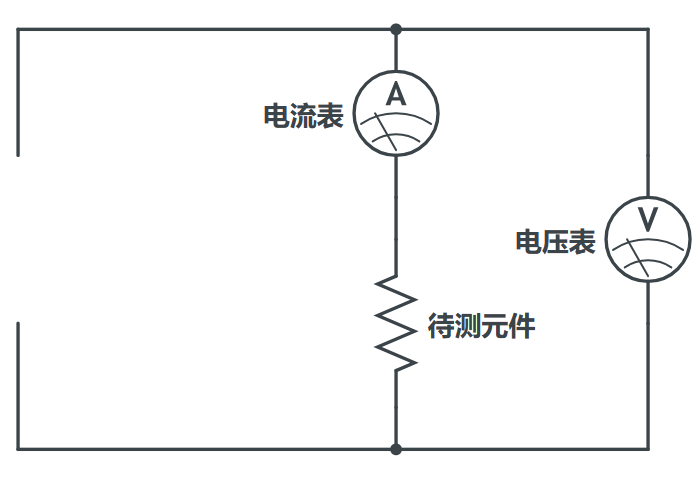
\includegraphics[width=0.3\textwidth]{fig1.png}}\hspace{5mm}
            \subfloat[电压表外接法]{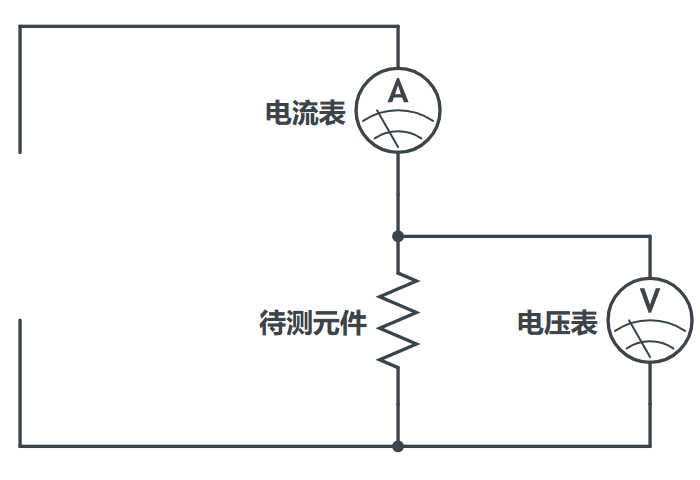
\includegraphics[width=0.3\textwidth]{fig2.png}}
        \end{figure}\par
        测量结果详见原始数据页,这里将不同方法得到的伏安特性曲线绘制出来:\par
        \begin{figure}[!ht]
            \caption{线性电阻元件}
            \subfloat[120\unit{\ohm} 电流表外接法 $i-u$]{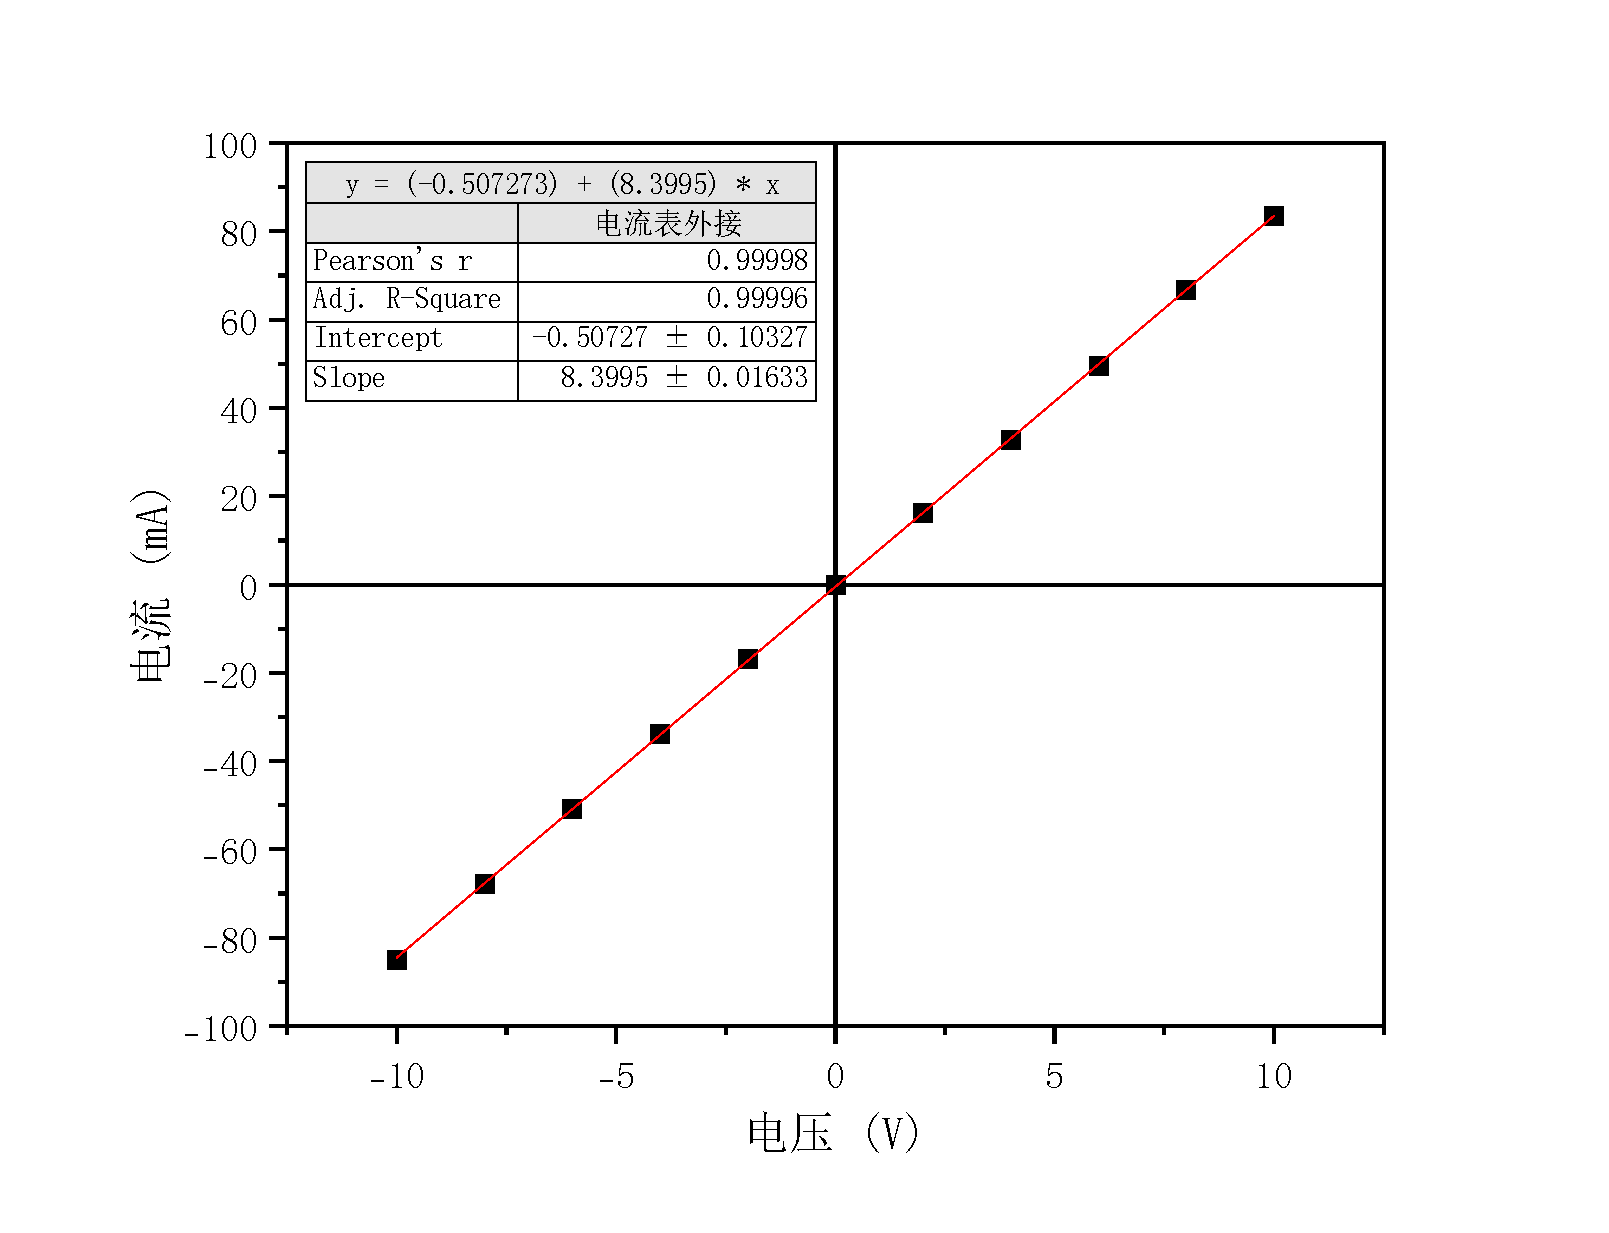
\includegraphics[width=0.45\textwidth]{res1.pdf}}
            \subfloat[120\unit{\ohm} 电压表外接法 $i-u$]{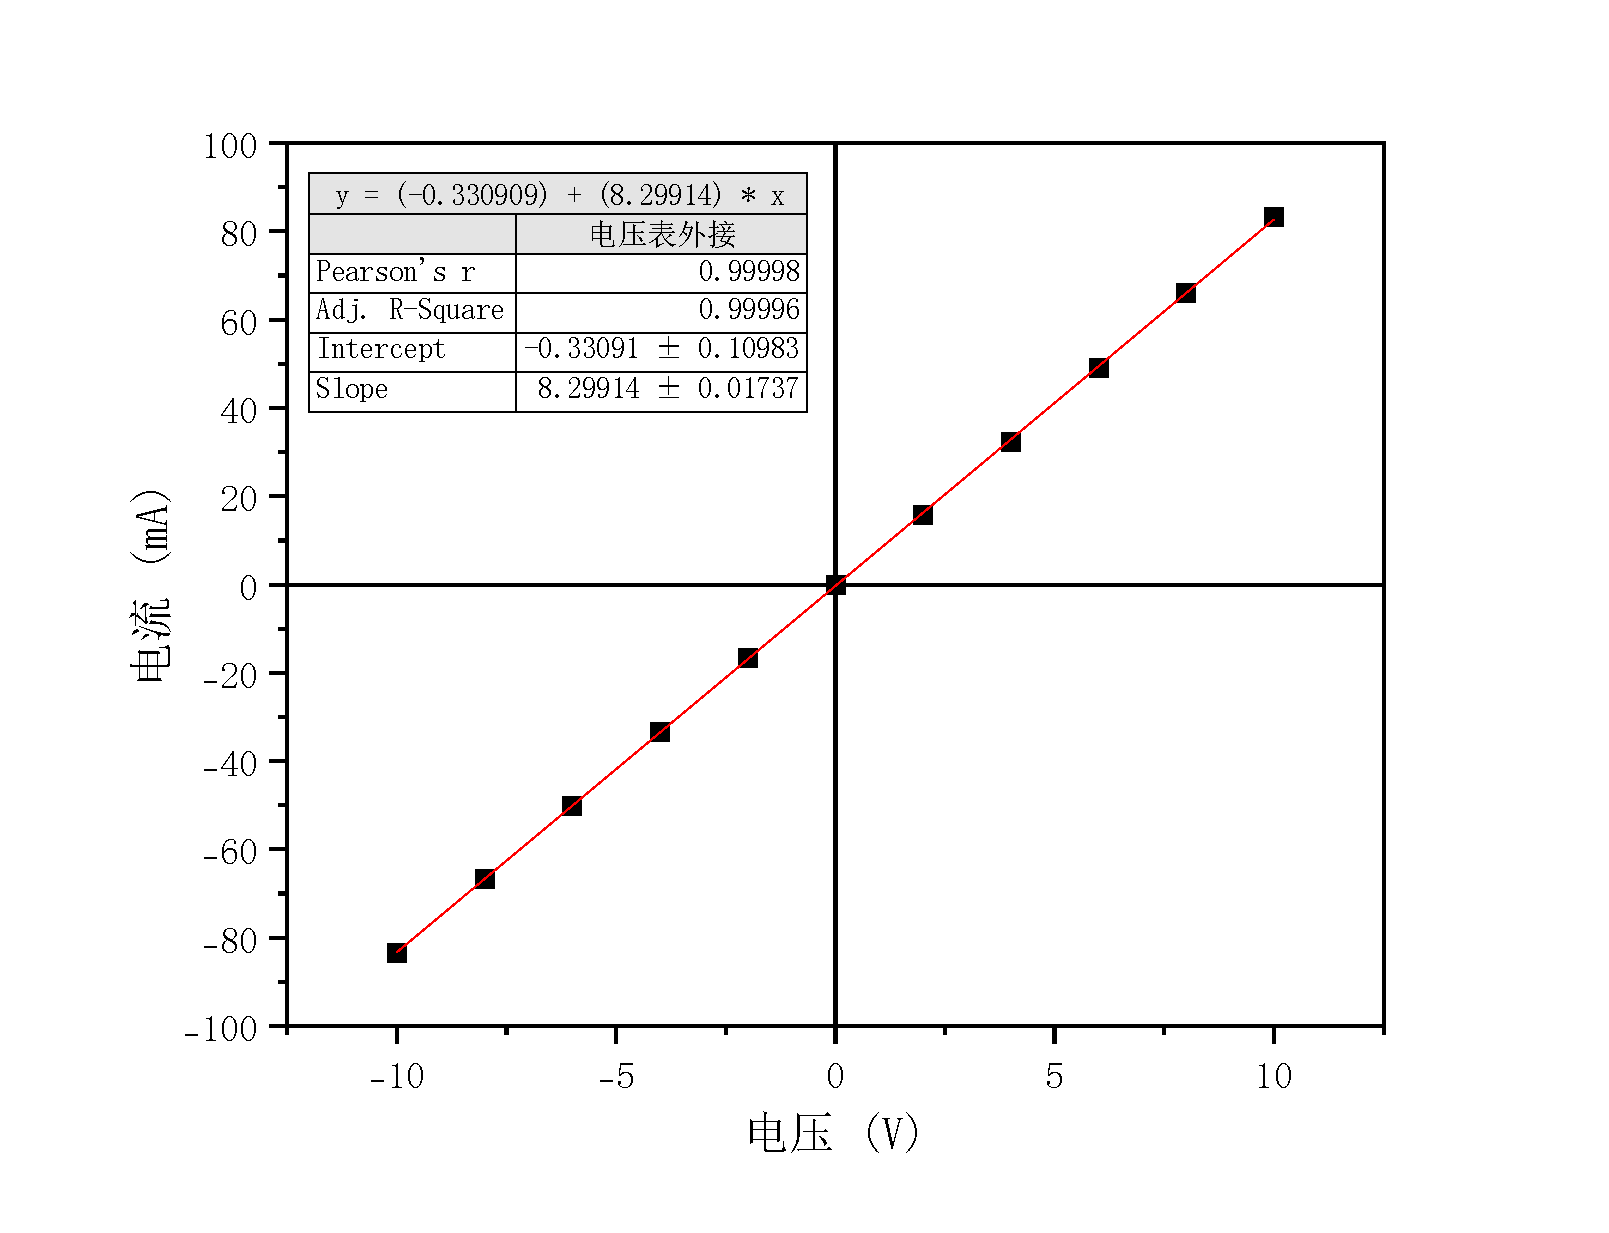
\includegraphics[width=0.45\textwidth]{res2.pdf}}\\
            \subfloat[120\unit{\ohm} 电流表外接法 $u-i$]{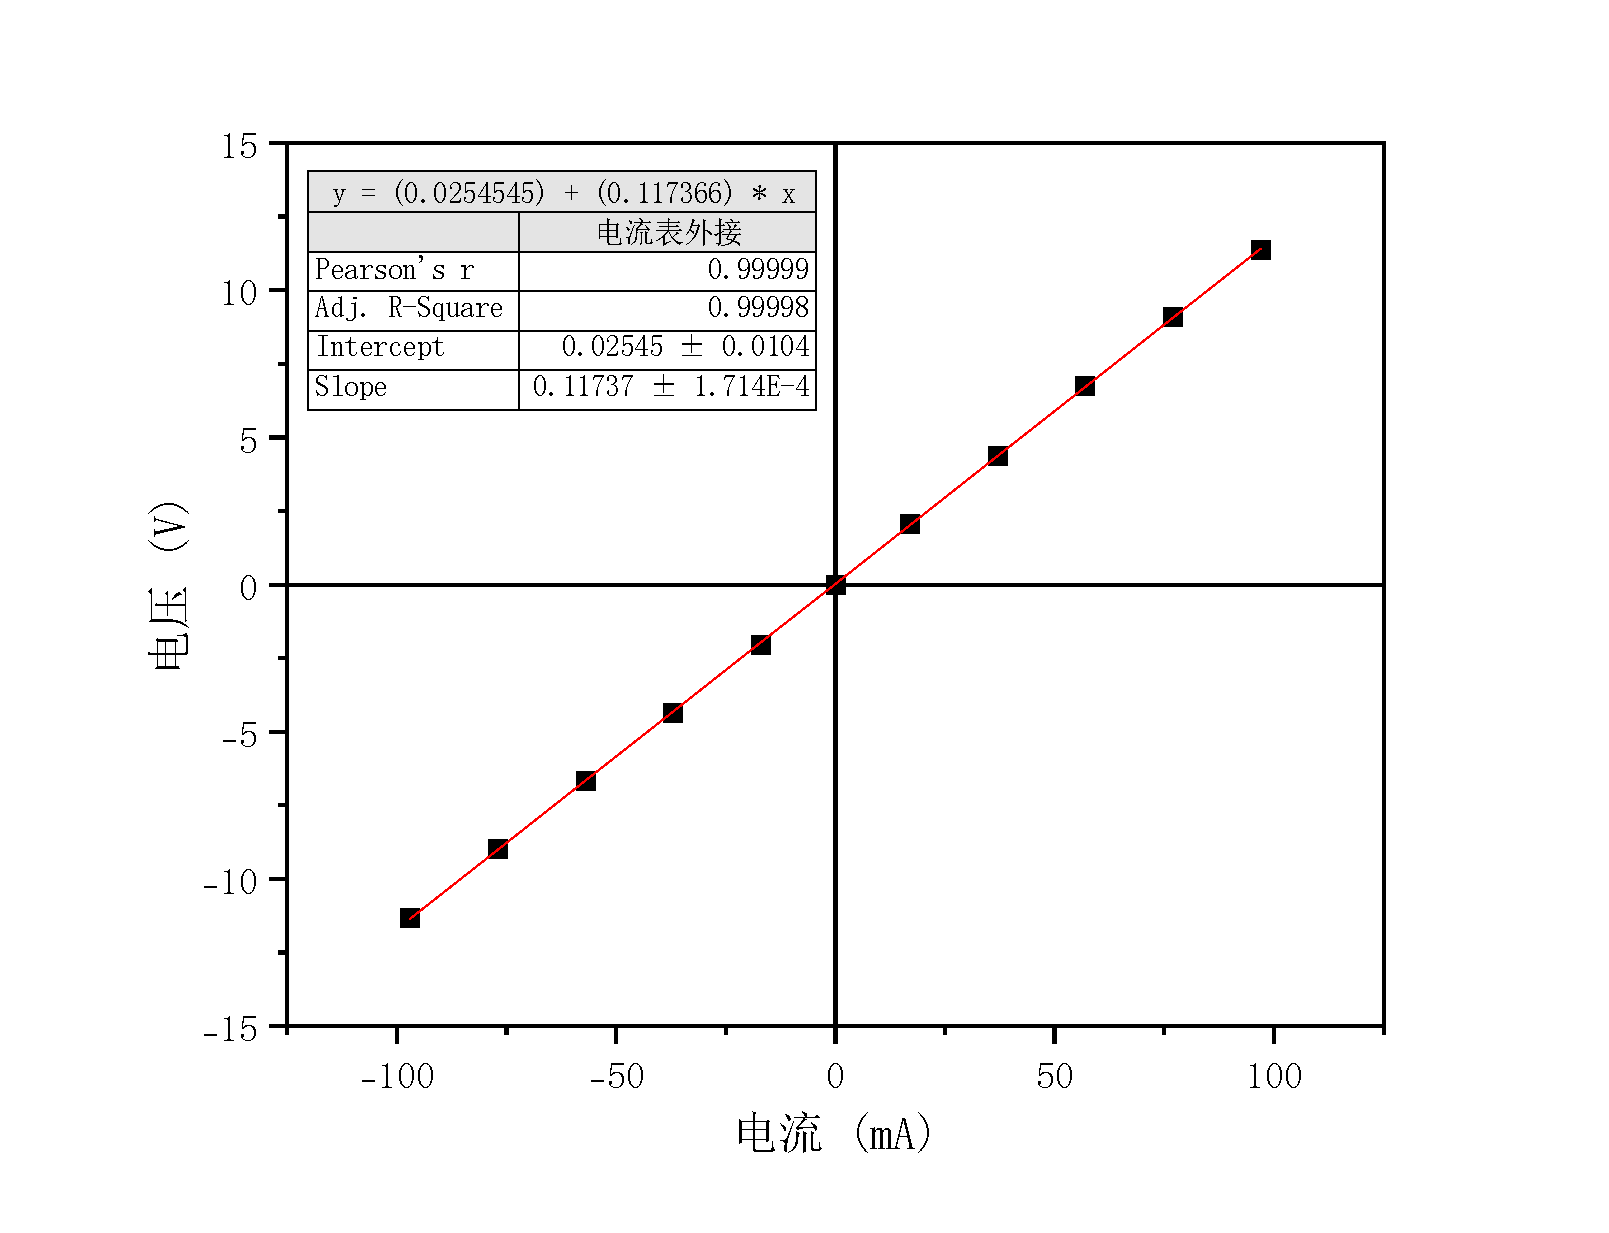
\includegraphics[width=0.45\textwidth]{res5.pdf}}
            \subfloat[120\unit{\ohm} 电压表外接法 $u-i$]{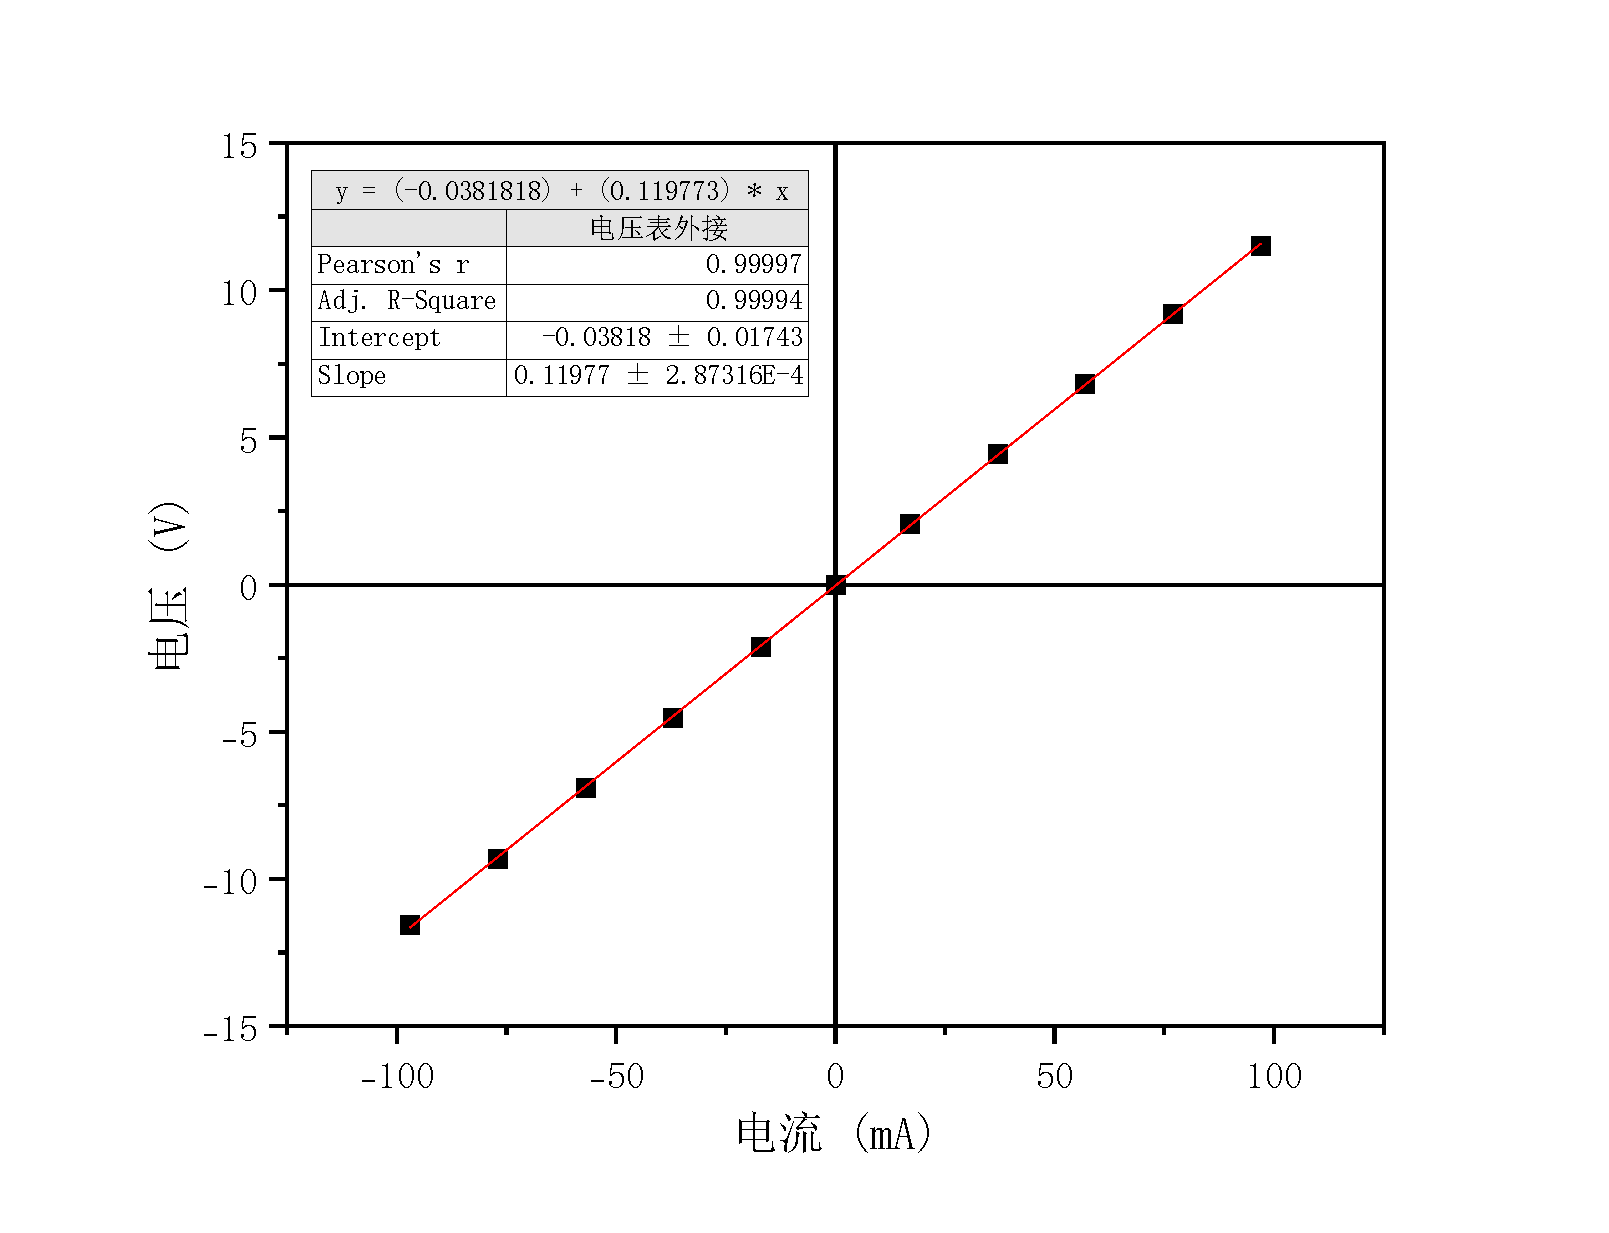
\includegraphics[width=0.45\textwidth]{res6.pdf}}\\
        \end{figure}\newpage
        \begin{figure}[!ht]
            \caption{非线性电阻元件}
            \subfloat[D3 $i-u$]{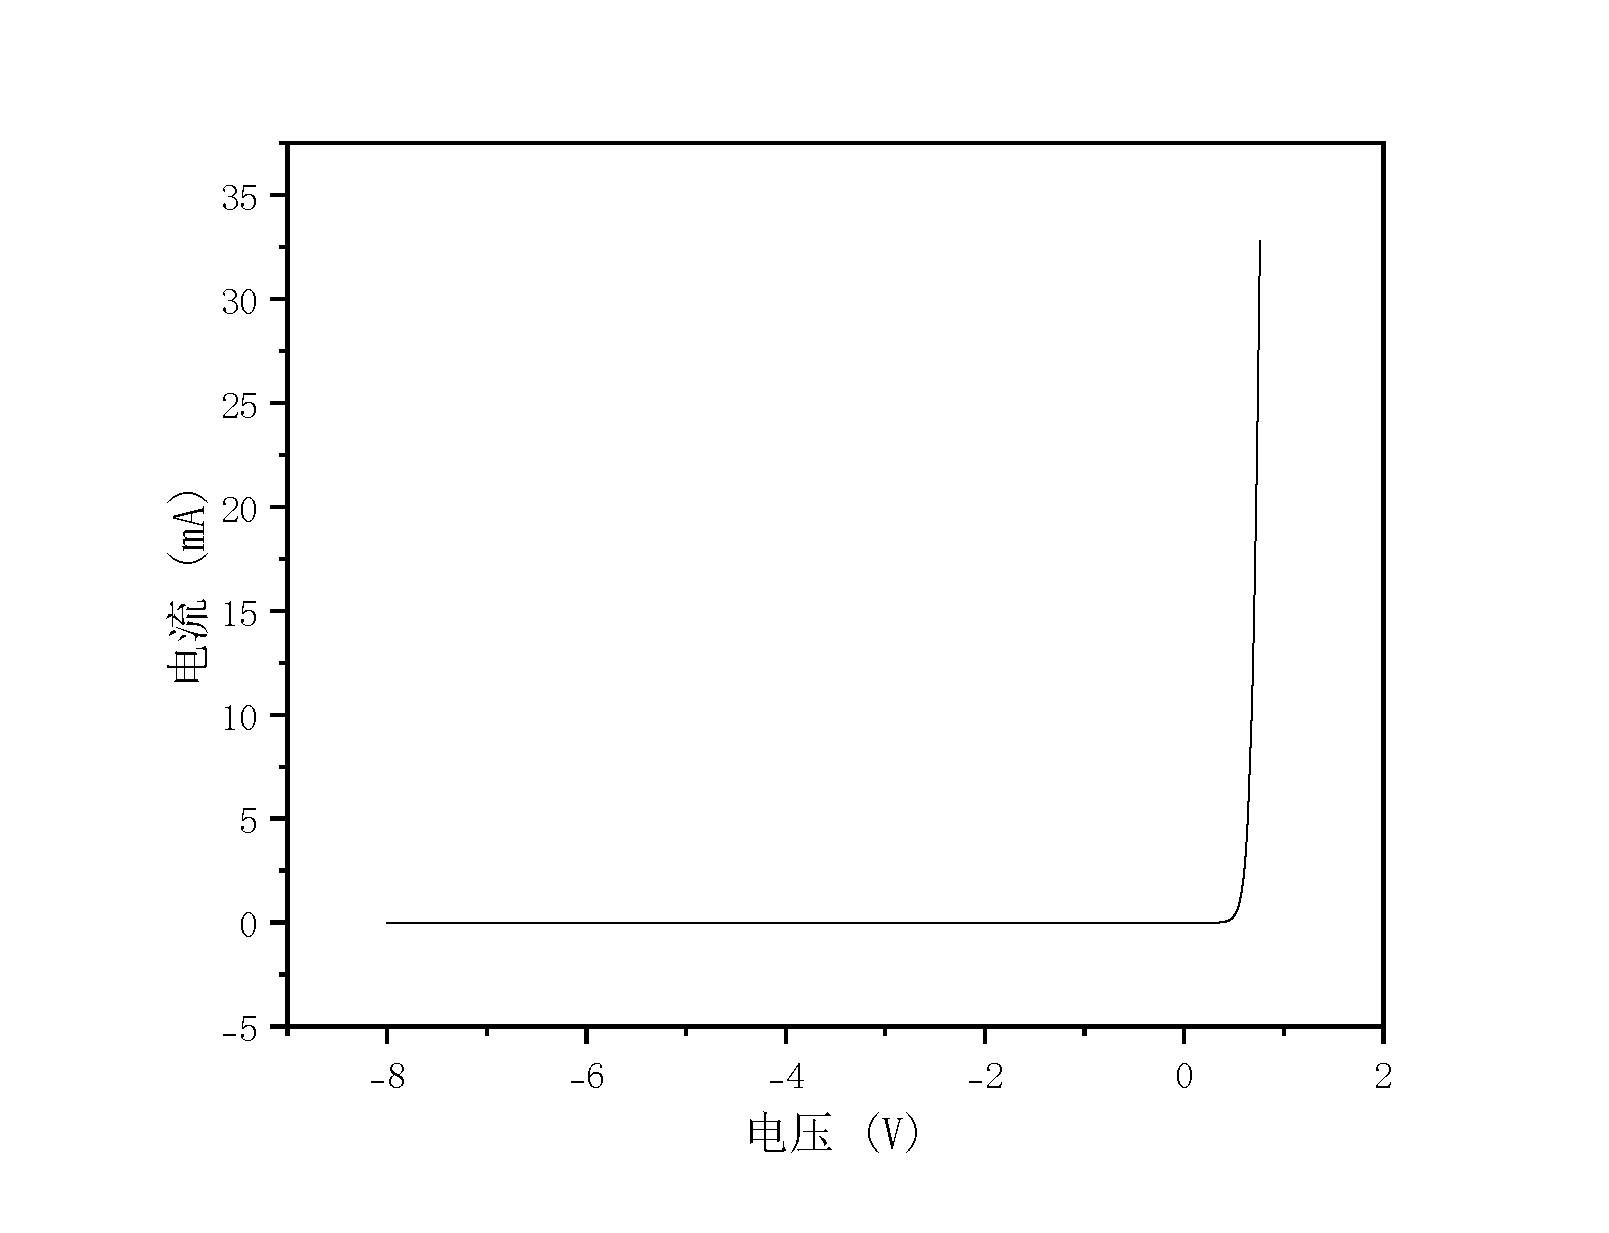
\includegraphics[width=0.45\textwidth]{res3.pdf}}
            \subfloat[D4 $i-u$]{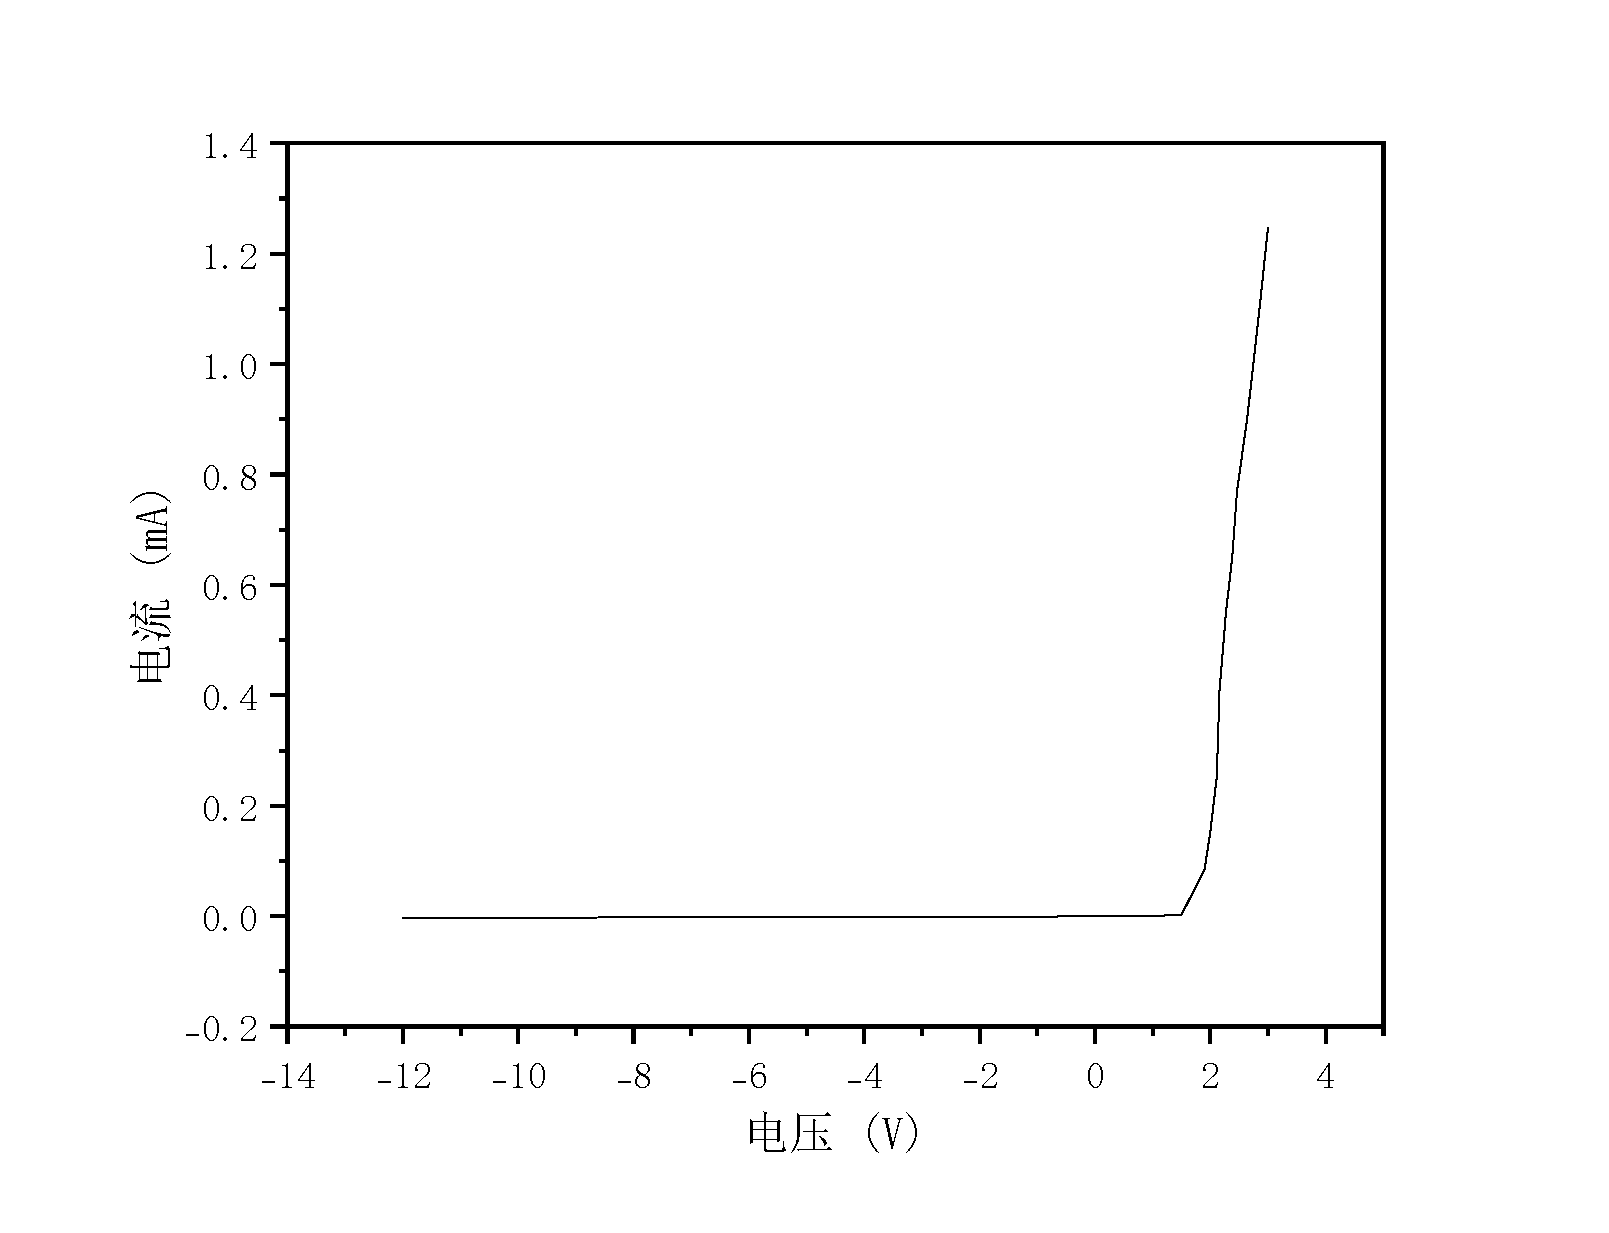
\includegraphics[width=0.45\textwidth]{res4.pdf}}\\
            \subfloat[D3 $u-i$]{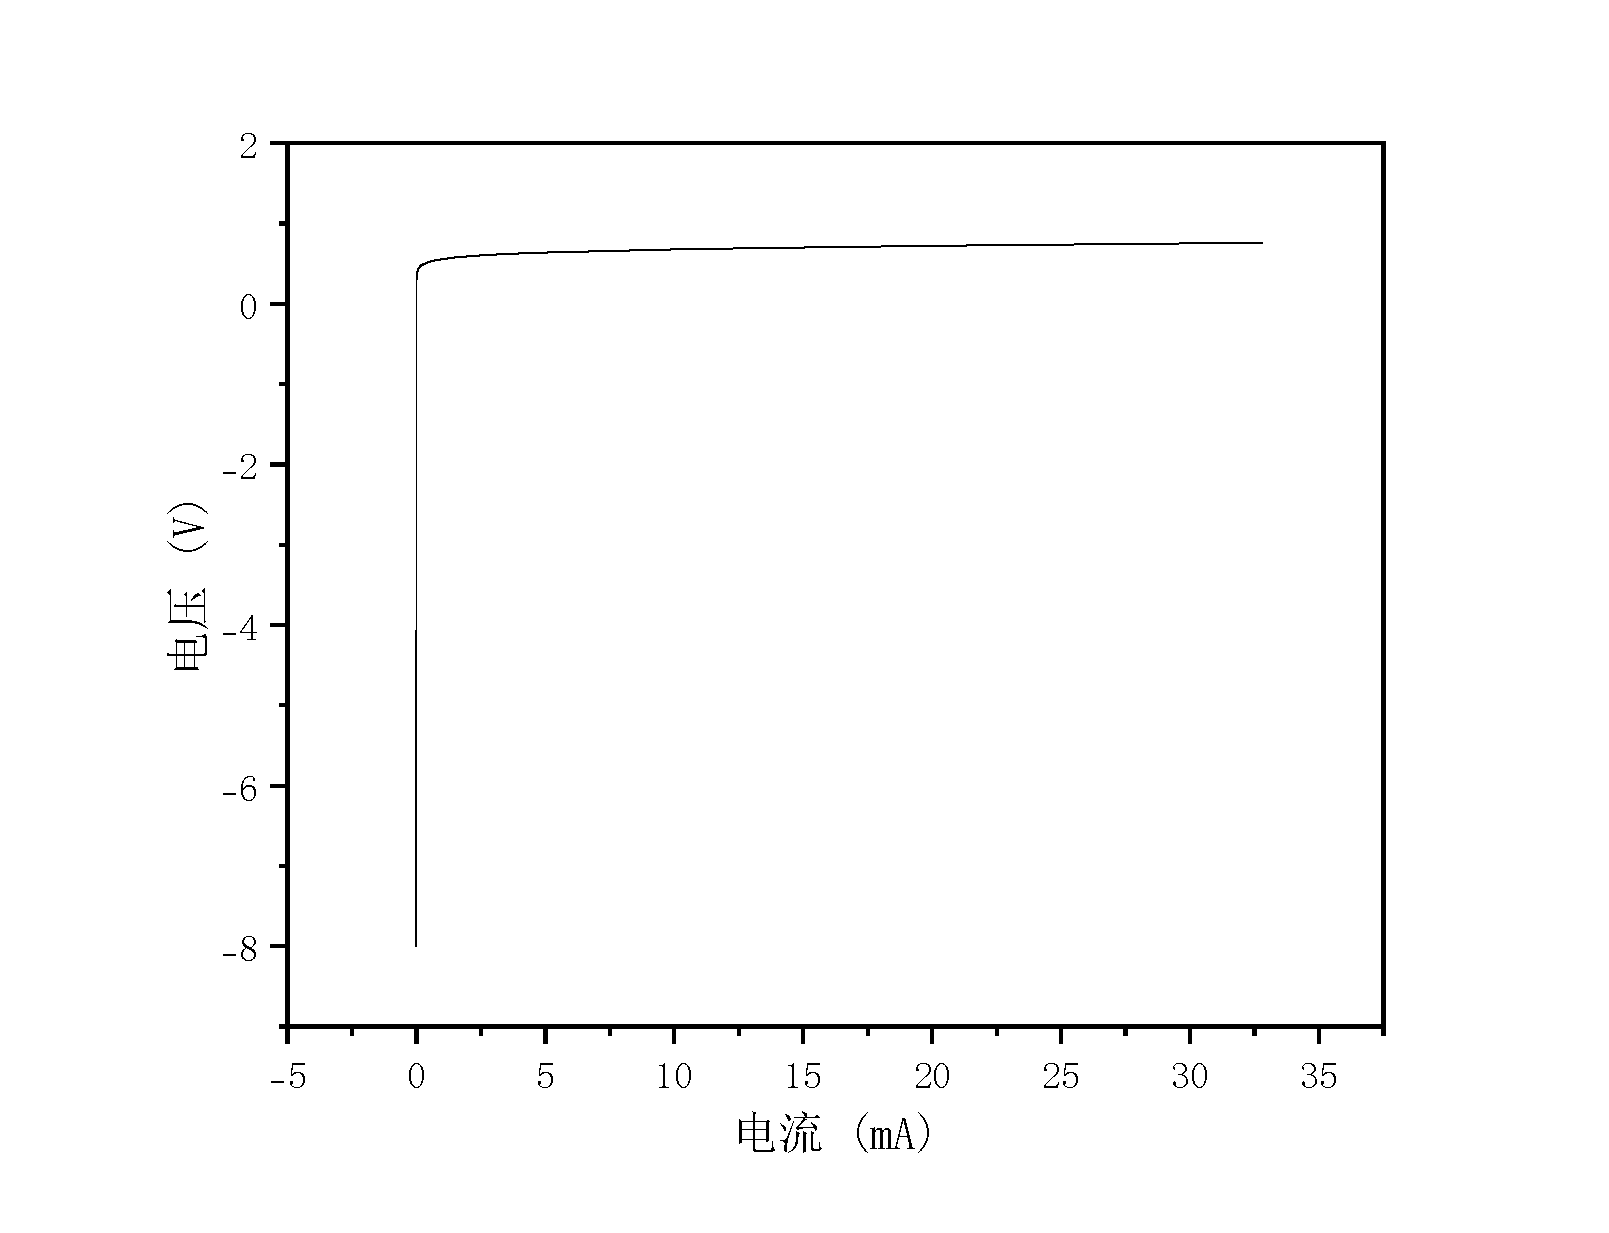
\includegraphics[width=0.45\textwidth]{res7.pdf}}
            \subfloat[D4 $u-i$]{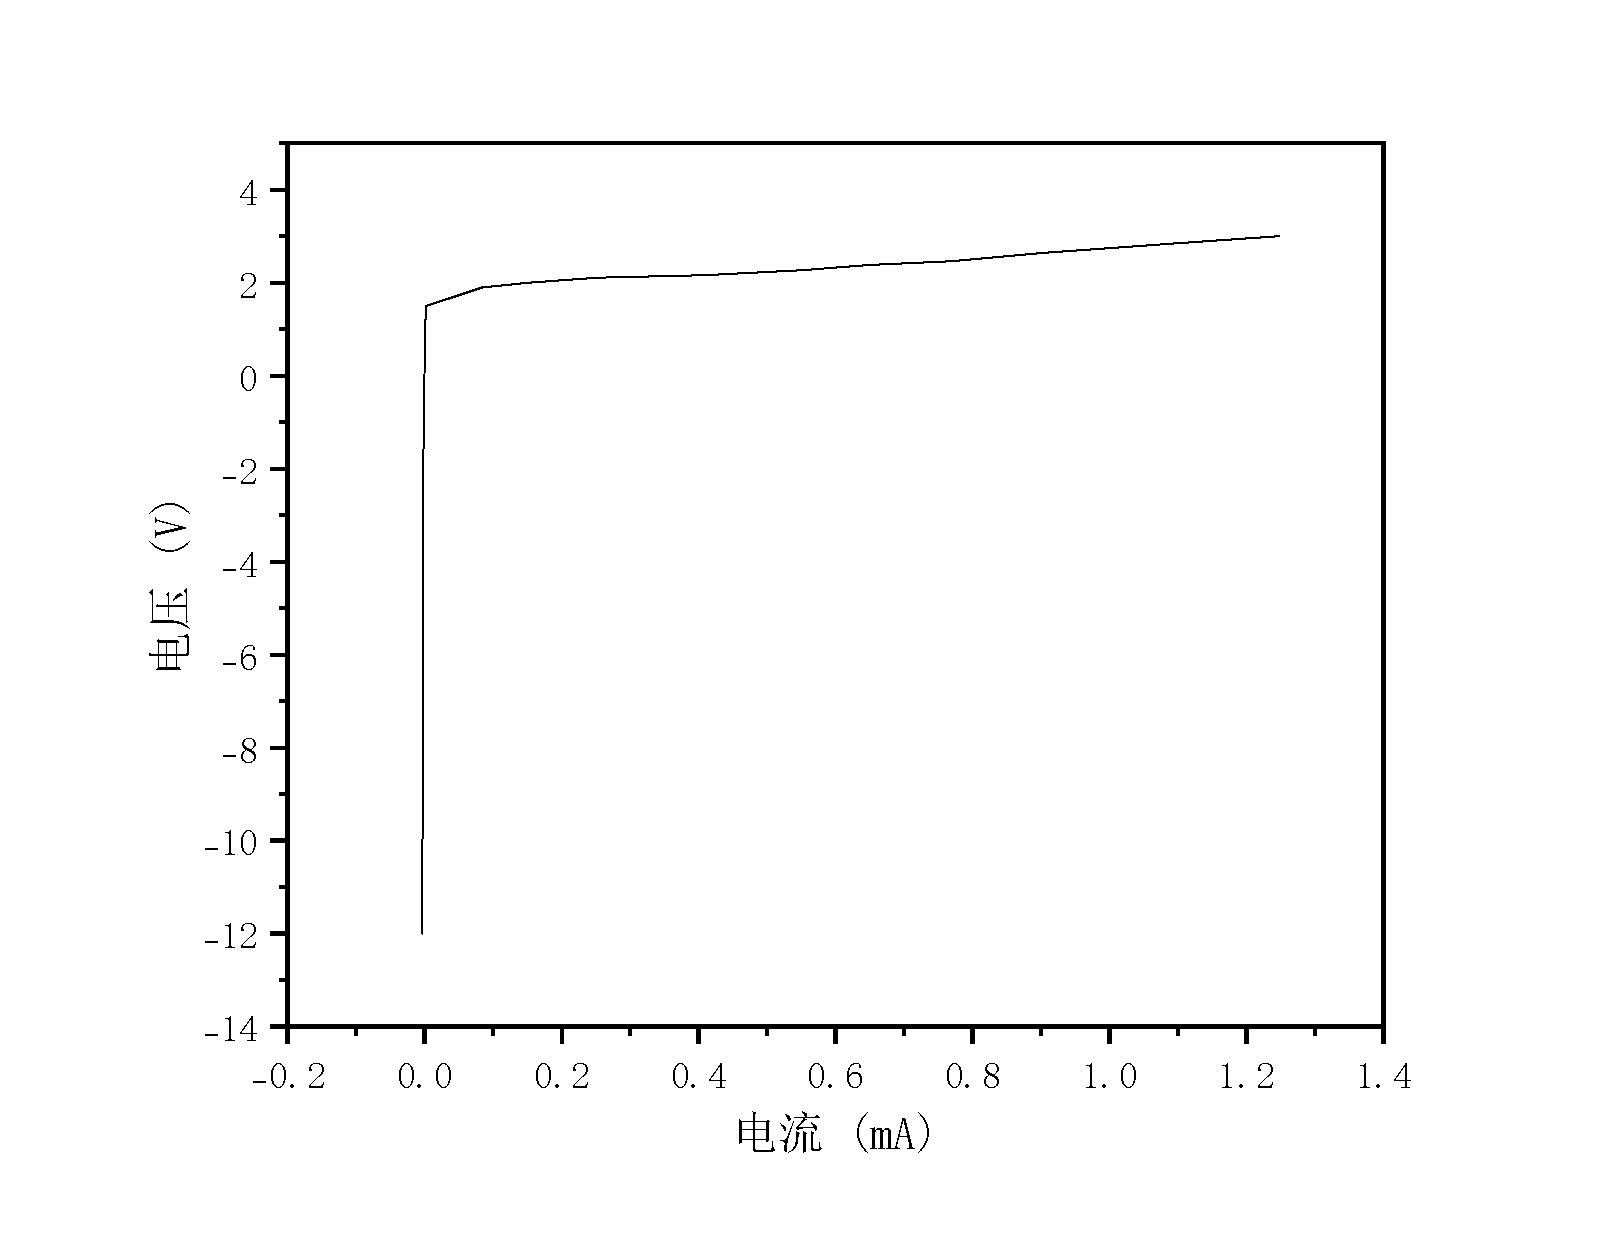
\includegraphics[width=0.45\textwidth]{res8.pdf}}\\
        \end{figure}\par
        对线性电阻元件拟合得到的电阻值:
        \begin{table}[!ht]
            \centering\begin{tabular}{c c c c}\toprule
                元件 & 测量方法 & 电阻 $R$ & 相对误差 \\ \midrule
                \multirow[c]{2}*{120\unit{\ohm}电阻} & 电流表外接 & $117.3 \pm 0.2$\unit{\ohm} & 2.25\% \\
                & 电压表外接 & $119.7 \pm 0.3$\unit{\ohm} & 0.25\% \\ \bottomrule
            \end{tabular}\caption{线性电阻元件电阻值}
        \end{table}\par
        事实上,对于非理想电流表和电压表,其分流和分压效果是不可以忽略的,若是将其视为理想的表,对于电流表外接法:此时电流表测得的电流是流过电阻和流过电压表的总和,在电压测量准确的情况下,实际算出的电阻应当偏小;而对于电压表外接法:此时电压表测得的电压是电阻和电流表的总和,在电流测量准确的情况下,实际算出的电阻应当偏大。结合本次实验得到的结果,可以认为该标称 120\unit{\ohm}的电阻实际值应当在\qrange{117.3}{119.7}{\unit{\ohm}}之间。\par
        对于 D3,D4 两个非线性电阻元件,可以在图上读出几个重要信息:
        \begin{enumerate}
            \item 这两个二极管元件具有很明显的单向性,反向时即使电压很高也没有电流通过
            \item 电压正向时存在一个最小的电压阈值可以使其导通,即在这一点后电阻由无穷大变为一个很低的值
        \end{enumerate}\par
        误差分析:本次实验所采用的仪器精度很高,实验结果所包含的误差中,仪器误差占比较小,并且从实验结果可以看到,此次实验测量的误差都很小,可以认为是实验操作较规范。其余具体的误差来源如下:
        \begin{enumerate}
            \item 实验箱上的待测元件与标称值本身存在误差,且长时间放置也会产生变化
            \item 测试线路上的电阻、寄生电容
            \item 测试当天的温度湿度导致的误差
            \item 引脚可能生锈而产生额外变化
        \end{enumerate}

\section{思考题}
    \subsection{线性电阻元件的两个特殊情况“开路”、“短路”的含义是什么?}
        开路又称断路,此时元件两端可能有电压但一定没有电流通过;短路则相反,此时元件相当于与导线并联,元件两端无电压,也没有电流通过。
    \subsection{试说明可调三端电阻最常见的三个用途,最好能画图说明}
        可调三端电阻即电位器,广泛运用在需要调节电流的场景,如调节灯光亮暗、音响声音大小、电机转速。以下是一个非常简单示例,用可调三端电阻实现灯光亮暗调节:
        \begin{figure}[!ht]
            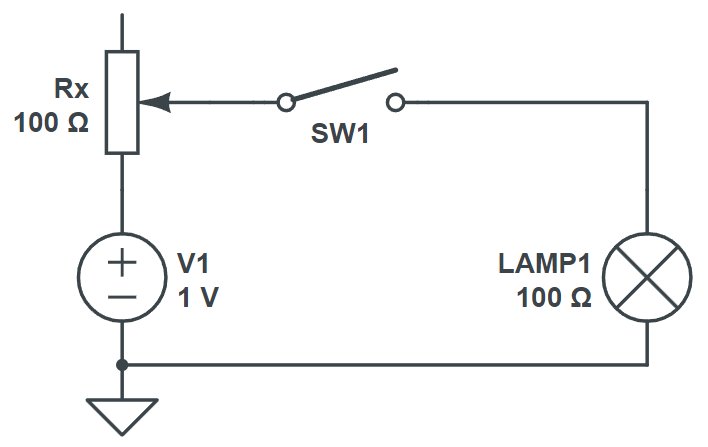
\includegraphics[width=0.6\textwidth]{thi1.png}
        \end{figure}\par
    \subsection{思考题3}
        电流表应与被测元件串联,电压表应与被测元件并联,电流表、电压表都有内阻,而电流表内阻应越小越好,电压表内阻应越大越好,这是因为电流表内阻越小,分压越小;电压表内阻越大,分流越少,在伏安法测量当中可以进一步缩小系统误差。
    \subsection{试分析接入电路的电流表内阻大、电压表内阻小时,对测试结果有何影响?}
        \begin{enumerate}
            \item 对于电流表外接法,此时电压表内阻变小会导致电压表分到的电流增大,内阻越小,测得的电流越偏离实际电流,结果越偏小。
            \item 对于电压表外接法,此时电流表内阻变大会导致电流表分到的电压增大,内阻越大,测得的电压越偏离实际电压,结果越偏大。
        \end{enumerate}
    \subsection{如果被测元件阻值小应采用电流表外接法不是电压表外接法?被测元件阻值大又应如何连接?为什么?}
        记电流表阻值为$R_A$,电压表阻值为 $R_V$。于是有:
        \begin{align*}
            \text{电压表外接法:}&R_{measure}=R_A+R_{real}\\
            \text{电流表外接法:}&R_{measure}=\frac{R_V R_{real}}{R_V+R_{real}}
        \end{align*}
        计算其相对误差,并令两个相对误差相等即可求出临界的 $R_{real}$ 对于两种方法来说误差一样。解得临界的 $R_{real}$ 为:$\sqrt{R_V R_{A}+R_A R_{real}}$ (一个近似解为高中时学过的 $\sqrt{R_V R_{A}}$)。故当 $R_{real}$ 大于临界值时,应当使用电压表外接法,反之则使用电流表外接法。
   
\section{实验心得}
    本次实验采取了多种方法来测量同一元件的阻值,实际上这些方法各有各的最佳使用场景,正如思考题最后一题推导出来的临界值。因此在实际测量中应当活用各种测量方法,找到系统误差最小的最优方案进行测量。
\newpage
\section{原始数据}
    \begin{figure}[!ht]
        \includegraphics*[width=0.9\textwidth]{data.jpg}
    \end{figure}
\end{document}